\documentclass{beamer}
% Required packages
\usepackage{amsmath}
\usepackage{physics}
\usepackage{graphicx}
\usepackage{siunitx}
\usepackage{xcolor}
% Set image search paths
\graphicspath{{../images/}{../../shared/images/}}

% Define custom colors for DS9 theme
\definecolor{ds9blue}{RGB}{25,25,112}
\definecolor{ds9gold}{RGB}{218,165,32}
\definecolor{ds9grey}{RGB}{105,105,105}
\definecolor{ds9red}{RGB}{178,34,34}
% Set up the Madrid theme with custom colors
\usetheme{Madrid}
\usecolortheme{whale}
\setbeamercolor{palette primary}{bg=ds9blue,fg=white}
\setbeamercolor{palette secondary}{bg=ds9grey,fg=white}
\setbeamercolor{palette tertiary}{bg=ds9gold,fg=black}
\setbeamercolor{palette quaternary}{bg=ds9red,fg=white}
\setbeamercolor{structure}{fg=ds9blue}
\setbeamercolor{title}{fg=ds9gold}
\setbeamercolor{subtitle}{fg=ds9gold}
\setbeamercolor{frametitle}{bg=ds9blue,fg=white}
\setbeamercolor{block title}{bg=ds9blue,fg=white}
\setbeamercolor{block body}{bg=ds9grey!20,fg=black}

% Title page configuration
\title[Electric Circuits]{PHYS11 CH:19.1-19.4}
\subtitle{Ohm's Law, Series \& Parallel Circuits, and Electric Power}
\author[Mr. Gullo]{Mr. Gullo}
\date[May 2025]{May, 2025}

\begin{document}

% Title slide
\begin{frame}
\titlepage
\end{frame}

% Table of contents
\begin{frame}
\frametitle{Outline}
\tableofcontents
\end{frame}

\section{Learning Objectives}

\begin{frame}
\frametitle{Learning Objectives}
By the end of this lesson, you will be able to:
\begin{itemize}
\item State and apply Ohm's law to simple circuits
\item Distinguish between series and parallel circuit configurations
\item Calculate equivalent resistance for resistors in series and parallel
\item Analyze current flow and voltage drops in different circuit configurations
\item Compute electric power dissipation in resistive elements
\end{itemize}
\end{frame}

\section{Ohm's Law}

\begin{frame}
\frametitle{Current and Resistance}
\begin{block}{Electric Current}
Electric current is the rate of charge flow:
\begin{align}
I = \frac{\Delta Q}{\Delta t}
\end{align}
where:
\begin{itemize}
\item $I$ is the current (measured in amperes, A)
\item $\Delta Q$ is the charge that passes (measured in coulombs, C)
\item $\Delta t$ is the time interval (measured in seconds, s)
\end{itemize}
\end{block}

\begin{block}{Definition of Ampere}
\begin{align}
1 \text{ A} = 1 \text{ C/s}
\end{align}
\end{block}
\end{frame}

\begin{frame}
\frametitle{Ohm's Law}
\begin{block}{Ohm's Law Statement}
For ohmic materials, the voltage drop along a path is proportional to the current that runs through the path, with resistance as the constant of proportionality.
\end{block}

\begin{block}{Mathematical Form}
\begin{align}
V = IR
\end{align}
where:
\begin{itemize}
\item $V$ is the voltage drop (measured in volts, V)
\item $I$ is the current (measured in amperes, A)
\item $R$ is the resistance (measured in ohms, $\Omega$)
\end{itemize}
\end{block}
\end{frame}

\begin{frame}
\frametitle{Ohm's Law}
\begin{alertblock}{}
\begin{figure}
    \centering
    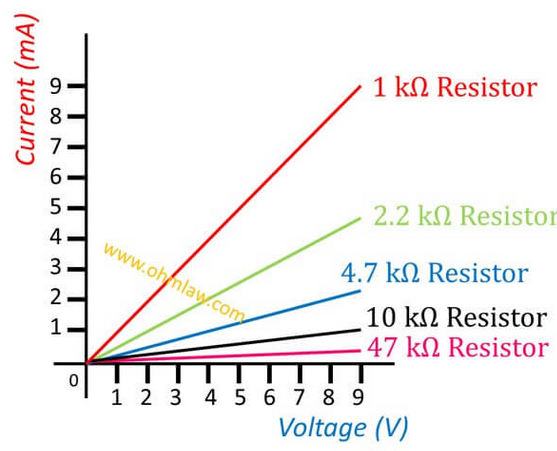
\includegraphics[width=0.7\linewidth]{ohmgr.png}
\end{figure}
\end{alertblock}
\end{frame}

\begin{frame}
\frametitle{Direct vs. Alternating Current}
\begin{columns}
\column{0.5\textwidth}
\begin{block}{Direct Current (DC)}
\begin{itemize}
\item Constant over time
\item Flows in one direction
\item Example: Batteries
\end{itemize}
\end{block}

\column{0.5\textwidth}
\begin{block}{Alternating Current (AC)}
\begin{itemize}
\item Alternates back and forth over time
\item Changes direction periodically
\item Example: Household electricity
\end{itemize}
\end{block}
\end{columns}

\begin{alertblock}{Current Types Visualization}
\begin{figure}
    \centering
    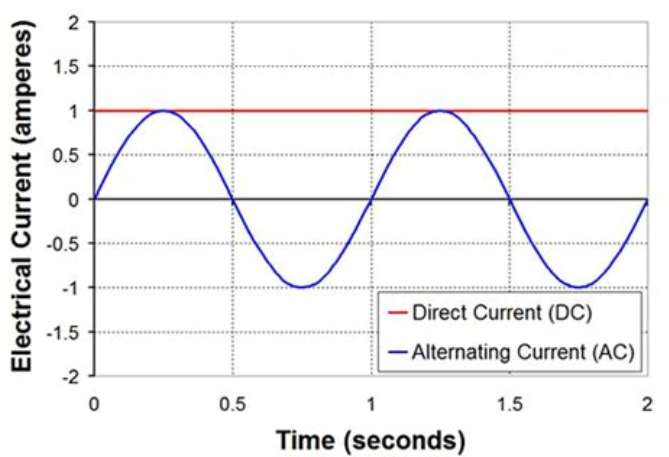
\includegraphics[width=0.5\linewidth]{cdfgrge.png}
\end{figure}
\end{alertblock}
\end{frame}

\section{Series Circuits}

\begin{frame}
\frametitle{Series Circuits: Characteristics}
\begin{block}{Definition}
Resistors in series are connected head to tail, forming a single path for current flow.
\end{block}

\begin{columns}
\column{0.6\textwidth}
\begin{block}{Key Properties}
\begin{itemize}
\item Same current flows through all resistors
\item Voltage drop can be different across each resistor
\item Voltage is the same at every point in a given wire
\item Total voltage equals sum of individual voltage drops
\end{itemize}
\end{block}

\column{0.4\textwidth}
\begin{alertblock}{Series Circuit}
\alert{}
\begin{figure}
    \centering
    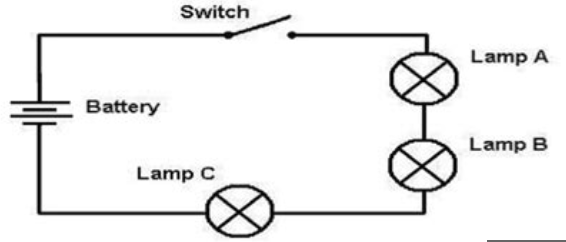
\includegraphics[width=1\linewidth]{srecrc.png}
\end{figure}
\end{alertblock}
\end{columns}
\end{frame}

\begin{frame}
\frametitle{Series Circuits: Equivalent Resistance}
\begin{block}{Equivalent Resistance Formula}
For $N$ resistors connected in series:
\begin{align}
R_{\text{equiv}} = R_1 + R_2 + \cdots + R_N
\end{align}
\end{block}

\begin{block}{Interpretation}
\begin{itemize}
\item The equivalent resistance is always greater than any individual resistance
\item Adding resistors in series increases the total resistance
\item Current is limited by the sum of all resistances
\end{itemize}
\end{block}


\end{frame}

\section{Parallel Circuits}

\begin{frame}
\frametitle{Parallel Circuits: Characteristics}
\begin{block}{Definition}
Resistors in parallel provide multiple paths for current flow, with one end of each resistor connected to a common point.
\end{block}

\begin{columns}
\column{0.6\textwidth}
\begin{block}{Key Properties}
\begin{itemize}
\item Same voltage across all resistors
\item Current through each resistor can differ
\item Total current equals sum of individual currents
\item More paths available for current flow
\end{itemize}
\end{block}

\column{0.4\textwidth}
\begin{alertblock}{Parallel Circuit}
\alert{}
\begin{figure}
    \centering
    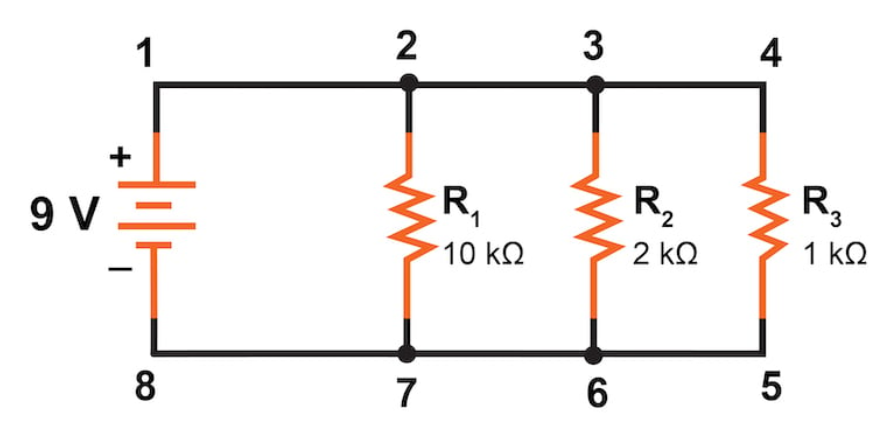
\includegraphics[width=1\linewidth]{prllrlrl.png}
\end{figure}
\end{alertblock}
\end{columns}
\end{frame}

\begin{frame}
\frametitle{Parallel Circuits: Equivalent Resistance}
\begin{block}{Equivalent Resistance Formula}
For $N$ resistors connected in parallel:
\begin{align}
\frac{1}{R_{\text{equiv}}} = \frac{1}{R_1} + \frac{1}{R_2} + \cdots + \frac{1}{R_N}
\end{align}
\end{block}

\begin{block}{Special Case: Identical Resistors}
For $N$ identical resistors each with resistance $R$ connected in parallel:
\begin{align}
R_{\text{equiv}} = \frac{R}{N}
\end{align}
\end{block}

\begin{block}{Interpretation}
\begin{itemize}
\item The equivalent resistance is always less than the smallest individual resistance
\item Adding resistors in parallel decreases the total resistance
\end{itemize}
\end{block}
\end{frame}

\section{Electric Power}

\begin{frame}
\frametitle{Electric Power: Basic Concept}
\begin{block}{Definition}
Electric power is the rate at which energy is transferred or converted in an electric circuit.
\end{block}

\begin{block}{Key Points}
\begin{itemize}
\item Electric power is dissipated in resistances of a circuit
\item Capacitors do not dissipate electric power
\item Power dissipation often manifests as heat
\item Measured in watts (W), where 1 W = 1 J/s
\end{itemize}
\end{block}
\end{frame}

\begin{frame}
\begin{alertblock}{Power Dissipation}
\begin{figure}
    \centering
    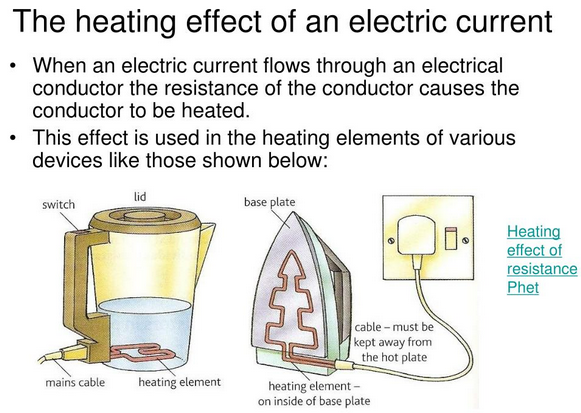
\includegraphics[width=1\linewidth]{reshet.png}
\end{figure}
\end{alertblock}
\end{frame}

\begin{frame}
\frametitle{Electric Power: Mathematical Expressions}
\begin{block}{Basic Power Formula}
Power is proportional to voltage and current:
\begin{align}
P = IV
\end{align}
\end{block}

\begin{block}{Alternative Expressions (Using Ohm's Law)}
Without current term:
\begin{align}
P = \frac{V^2}{R}
\end{align}

Without voltage term:
\begin{align}
P = I^2R
\end{align}
\end{block}
\end{frame}

\begin{frame}
\begin{alertblock}{Equivalent Expressions}
\begin{figure}
    \centering
    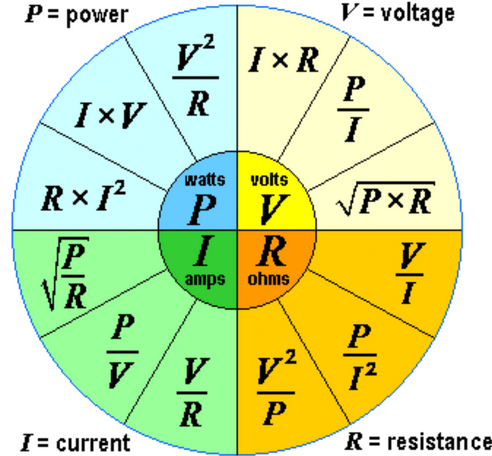
\includegraphics[width=0.7\linewidth]{pvri.png}
\end{figure}
\end{alertblock}
\end{frame}

\section{Examples}

\begin{frame}
\frametitle{I Do: Ohm's Law Example}
\begin{exampleblock}{Problem}
A resistor with resistance $R = 10 \, \Omega$ is connected to a voltage source of $V = 12 \, \text{V}$. Calculate the current flowing through the resistor.
\end{exampleblock}
\pause
\begin{block}{Solution}
Using Ohm's law: $V = IR$

Rearranging to solve for current: $I = \frac{V}{R}$

Substituting the values:
\begin{align}
I &= \frac{12 \, \text{V}}{10 \, \Omega} \\
&= 1.2 \, \text{A}
\end{align}

Therefore, the current flowing through the resistor is $1.2 \, \text{A}$.
\end{block}
\end{frame}

\begin{frame}
\frametitle{We Do: Series Circuit Analysis}
\begin{exampleblock}{Problem}
Three resistors are connected in series: $R_1 = 5 \, \Omega$, $R_2 = 10 \, \Omega$, $R_3 = 15 \, \Omega$. If connected to a $30 \, \text{V}$ source:
\begin{enumerate}
\item Calculate the equivalent resistance
\item Find the current through the circuit
\item Calculate the voltage drop across each resistor
\end{enumerate}
\end{exampleblock}

\begin{block}{Partial Solution}
1. Equivalent resistance:
\begin{align}
R_{\text{equiv}} &= R_1 + R_2 + R_3 \\
&= 5 \, \Omega + 10 \, \Omega + 15 \, \Omega \\
&= 30 \, \Omega
\end{align}


\end{block}
\end{frame}

\begin{frame}
\frametitle{We Do: Series Circuit Analysis (continued)}
\begin{block}{Complete the Solution}


2. Circuit current:
\begin{align}
I &= \frac{V}{R_{\text{equiv}}} \\
&= \frac{30 \, \text{V}}{30 \, \Omega} \\
&= 1 \, \text{A}
\end{align}
3. Voltage drops across each resistor:

For $R_1$: $V_1 = I \times R_1 = 1 \, \text{A} \times 5 \, \Omega = $ ?

For $R_2$: $V_2 = I \times R_2 = 1 \, \text{A} \times 10 \, \Omega = $ ?

For $R_3$: $V_3 = I \times R_3 = 1 \, \text{A} \times 15 \, \Omega = $ ?
\\
Let's work through these calculations together.
\end{block}


\end{frame}

\begin{frame}
\frametitle{You Do: Parallel Circuit Problem}
\begin{exampleblock}{Problem}
Three resistors are connected in parallel: $R_1 = 6 \, \Omega$, $R_2 = 12 \, \Omega$, $R_3 = 4 \, \Omega$. If connected to a $24 \, \text{V}$ source:
\begin{enumerate}
\item Calculate the equivalent resistance
\item Find the total current from the source
\item Calculate the current through each resistor
\end{enumerate}
\end{exampleblock}

Work on this problem independently, and we'll review the solution together afterward.
\end{frame}

\section{Summary}

\begin{frame}
\frametitle{Key Concepts Summary}
\begin{columns}
\column{0.5\textwidth}
\begin{block}{Ohm's Law}
\begin{itemize}
\item $V = IR$
\item Linear relationship for ohmic materials
\end{itemize}
\end{block}

\begin{block}{Series Circuits}
\begin{itemize}
\item Same current through all resistors
\item $R_{\text{equiv}} = R_1 + R_2 + \cdots + R_N$
\end{itemize}
\end{block}

\column{0.5\textwidth}
\begin{block}{Parallel Circuits}
\begin{itemize}
\item Same voltage across all resistors
\item $\frac{1}{R_{\text{equiv}}} = \frac{1}{R_1} + \frac{1}{R_2} + \cdots + \frac{1}{R_N}$
\end{itemize}
\end{block}

\begin{block}{Electric Power}
\begin{itemize}
\item $P = IV = I^2R = \frac{V^2}{R}$
\end{itemize}
\end{block}
\end{columns}
\end{frame}

\begin{frame}
\frametitle{Practice Questions}
\begin{block}{Consider This}
\begin{enumerate}
\item How does adding more resistors in series affect the total current in a circuit?
\item Why is the equivalent resistance in a parallel circuit always less than the smallest individual resistor?
\item In what ways can you reduce power consumption in an electrical circuit?
\item How does current distribute in a parallel circuit? Why?
\end{enumerate}
\end{block}

\begin{block}{Next Steps}
We will explore more complex circuit configurations and apply these principles to practical problems in our next lesson.
\end{block}
\end{frame}

\end{document}